\documentclass{article}
\usepackage[utf8]{inputenc}
\usepackage[spanish]{babel}
\usepackage{listings}
\usepackage{graphicx}
\graphicspath{ {images/} }
\usepackage{cite}



\begin{document}

\begin{titlepage}
    \begin{center}
        \vspace*{1cm}
            
        \Huge
        \textbf{Informe de Análisis y Diseño Parcial 1}
            
        \vspace{0.5cm}
        \LARGE
        %Subtítulo
            
        \vspace{1.5cm}
            
        \textbf{YESIKA MILENA CARVAJAL DÍAZ}
        \textbf{NICOLL CAROLINE CHAZATAR}\\
        \textbf{ANDRÉS FELIPE ZULUAGA ORTIZ}
            
        \vfill
            
        \vspace{0.8cm}
            
        \Large
        Departamento de Ingeniería Electrónica y Telecomunicaciones\\
        Universidad de Antioquia\\
        Medellín\\
        21 de Febrero de 2022
            
    \end{center}
\end{titlepage}

\tableofcontents
\newpage

\section{INTRODUCCIÓN}
En este documento se presenta el informe completo y detallado del sistema de transmisión y recepción de datos del parcial 1 del curso de Informática II. Este documento es la implementación al proyecto parcial al cual se le hizo el análisis anteriormente.\\

Se realiza un sistema de transmisión y recepción de datos utilizando un circuito integrado 74HC595 para la paralelización de datos mandados previamente desde el arduino transmisor utilizando una señal de reloj para la recolección de estos; se utilizan circuitos integrados de compuertas lógicas inversoras y AND para la verificación de la clave, por tanto la generación de la señal de bandera que se ingresa al arduino receptor. \\

En el arduino transmisor se generan la señal de los datos, y dos señales para la recolección adecuada de los datos, una que da razón del tiempo por bit y la otra del tiempo por Byte, y en el circuito receptor se almacena el dato solicitado, en este caso es el mayor dato de los cinco números anteriores a la clave.


\section{RESÚMEN}
El informe busca obtener herramientas y conocimiento que ayuden a realizar el proyecto del curso de Informática II. Se analiza a profundidad el sistema de comunicación completo, logrando  establecer la transmisión de los datos entre transmisor y receptor mediante la señal de reloj,  haciendo uso del lenguaje en C++, Arduino, la plataforma Tinkercad y circuitos integrado para ello.


\section{OBJETIVOS}

\subsection{GENERAL}

Adquirir conocimientos de sistemas de transmisión por medio de sistemas integrados.

ayúdeme herramientas y conocimientos de apoyo para el análisis teórico del desarrollo del proyecto parcial.

\subsection{ESPECÍFICOS}

\begin{itemize}

        \item Desarrollar la capacidad de solución de problemas.
        
        \item Adquirir conocimientos en la utilización de Arduino.
        
        \item Entender sobre la interconexión entre Arduinos y entre arduinos con circuitos integrados.
        
        \item Manejar adecuadamente la plataforma de Tinkercad.
        
        \item Entender el uso del circuito integrado 74HC595.
        
        \item Comprender la utilización y la utilidad de las compuertas lógicas y de sus circuitos integrados.
        
\end{itemize}

\section{METODOLOGÍA}

\subsection{El proyecto se divide en 6 bloques:}

\begin{enumerate}
\item PC1: Recibe los datos vía serial y es el encargado de enviar los datos al primer Arduino.

\item Sistema de generación de información serial:  Este es el primer Arduino, el cual recibe la información que envía el PC1, y envía señal de datos y reloj. Los cuáles reciben el segundo Arduino, y el sistema de paralelización.

\item Sistema que paraleliza los datos:  En este bloque, se paraleliza la información de un byte, es decir, esta recoge un byte y lo separa en 8 bits independientes. Los 8 bits independientes entran paralelamente al circuito de verificación de la banda (sistema de desencriptación). La paralelización de los datos se realiza por medio del circuito integrado 74HC595.

\item Sistema de desencriptación: Este sistema recibe los datos binarios paralelizados y con respecto a estos se genera de salida una bandera. Si la bandera es verdadera, significa que el próximo byte será el mensaje real. Este sistema se crea con base al byte que verifica el ingreso del mensaje real, y se realiza con compuertas lógicas.

\item Sistema de recepción: Este sistema tiene tres entradas: los datos, la señal del reloj y la bandera de verificación del mensaje real. Los datos y la señal del reloj se ingresan desde el sistema de generación de información serial, y la bandera entra desde el sistema de desencriptación. El sistema de recepción almacena el dato correspondiente al mensaje real para posteriormente entregarlo al Arduino 2. La señal del reloj sirve para indicarle al sistema de recepción en qué momento empieza la recolección del mensaje real, la cual es de 8 flancos de subida o de bajada del reloj después de la activación de la bandera. Este bloque se encuentra en el Arduino 2.
PC2: Este bloque recibe la señal del mensaje real, desde el sistema de recepción, y lo reproduce en una pantalla LCD.

\end{enumerate}


\subsection{Análisis del parcial}
	
Primero se crea el código con el cual generaremos los datos que saldrán desde el PC1 hacia el primer Arduino, El arduino de transmisión recibe los datos y los transforma a binario.\\

Luego se crea la conexión entre ambos arduinos en Tinkercad y de manera simultánea se conecta el circuito integrado 74HC595 para paralelizar el binario.
Después se crea el código de cada arduino. 
Posteriormente se hace uso de las compuertas lógicas para verificar la bandera que recibe el arduino 2; esto se hace en el código de arduino.\\

Luego de conectar el PC2 (Pantalla LCD), y completar el circuito, se implementa una serie de pruebas para verificar el correcto funcionamiento del sistema de comunicación. 


\section{DESARROLLO}

Inicialmente para del desarrollo del proyecto se realiza prototipos de cada sección del sistema para posteriormente unir estas secciones y lograr resolver el proyecto de manera mas analítica.

\subsection{Circuito integrado 74HC595}
El circuito integrado es útil para la realización de la práctica en la creación del bloque Sistema que paraleliza los datos. El 74HC595 nos ayuda a paralelizar los bytes en sus 8 puertos de salida para que estos entren al Sistema de desencriptación.\\

Los pines de alimentación del integrado son el pin 8 para tierra y 16 para Vcc.\\

Se debe generar una diferencia de potencial en los pines MA y OE para habilitar las salida del integrado, por lo que el pin OE se conecta a tierra y MA a Vcc.\\

Los pines SH-CP(11), DS(14), ST-CP(12) controlan el ingreso de los bits que se reproducen en las salidas del integrado. El pin DS da el valor del bit, el SH-CP es la señal para tomar el bit de DS, y ST-CP muestra los bits almacenados previamente en las salidas del integrado. Las señales reproducidas inician desde la salida Q0 hasta Q7, que corresponden respectivamente a los pines 15 y 1-7. \cite{youtube}\\

Para el uso del circuito integrado independiente se realiza el monje de la figura 1, en donde el switch nos da el valor del bit, el botón izquiedo almacena el bit, y el botón derecho manda la señal al circuito para que los bits sean visibles.

\newpage

\begin{figure}[h]
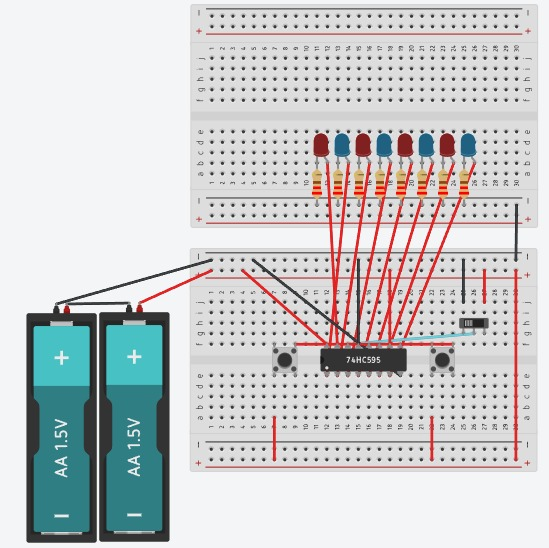
\includegraphics[width=7cm]{74HC595.jpg}
\centering
\caption{Circuito independiente 74HC595.}
\label{fig:74HC595.jpg}
\end{figure}
\cite{punto1}\\


\subsection{Comunicación entre Arduinos}
Para realizar la comunicación entre arduinos realizamos dos señales en el arduino transmisor (Arduino 1), las cuales son la señal de datos y la del reloj. \\

Para las señales de datos se utilizaron varias señales de prueba. Las señales de prueba para los datos fueron las siguientes:
\begin{itemize}
\item 01110010
\item 00110101
\item 10001100
\item 11111101010100101
\end{itemize}

La lectura de los datos se hará con cada flanco de subida del reloj.\\

Las señales de prueba se realizaron en el loop de Arduino y se utilizaron funciones delay. Los tiempos de delay se utilizan para entender cuándo se deben hacer modificaciones tanto en las señales de datos como en las del reloj.\\

Por ejemplo, para la primera señal de prueba para los datos, las señales de datos y de reloj se pueden observar como las señales de la figura 2, en donde t2 corresponde al tiempo entre la generación del bit de la señal de dato y el flanco de subida del reloj, y t1 corresponde al periodo de la señal de reloj.\\

\begin{figure}[h]
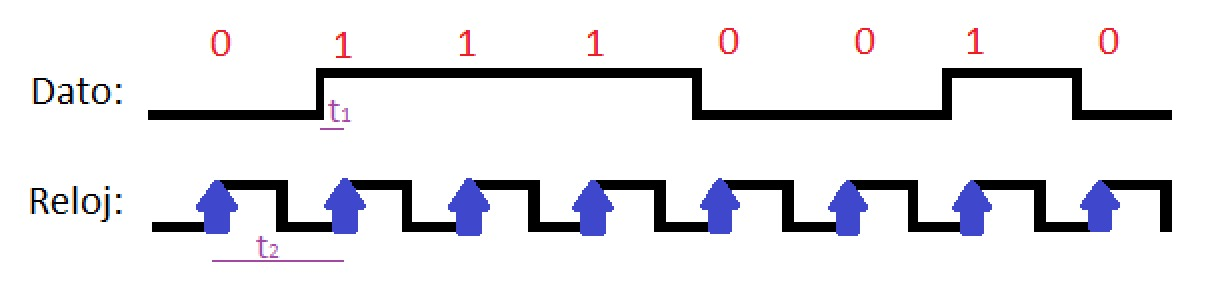
\includegraphics[width=11cm]{Prueba_datos_y_clock.jpeg}
\centering
\caption{Señales para la primera prueba de la señal de dato}
\label{fig:Prueba_datos_y_clock.jpeg}
\end{figure}

Para el t2 de la prueba, su valor es de 250 milisegundo. Se utilizan 125 milisegundos para el valor en alta y 125 milisegundos en baja. Para t1 se utiliza un valor de 25 milisegundos.\\


Para la interconexión entre los arduinos se realiza el monje de la figura 3, en donde en el arduino 1 el puerto 6 es la señal del reloj, el puerto 7 es la del bit a recolectar, y el puerto 6 del arduino 2 es el bit que se recibió visto como flanco.


\begin{figure}[h]
\includegraphics[width=6cm]{interconexión del arduino.PNG}
\centering
\caption{Interconexión de los Arduinos}
\label{fig:interconexión del arduino.PNG}
\end{figure}
\cite{punto2}\\

Basados en la figura 2, se realizan los códigos en Arduino.\\


Las figuras 4, 5 y 6 muestran el código en el arduino de transmisión y figura 7 muestra el código en el arduino de recepción.\\

\newpage

\begin{figure}[h]
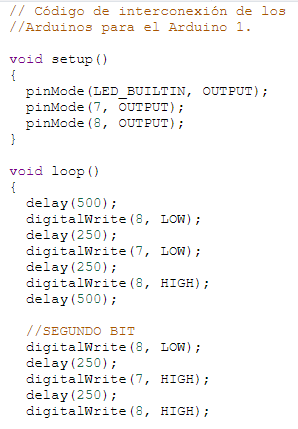
\includegraphics[width=6cm]{codigo_arduino1_1.PNG}
\centering
\caption{Primera parte del código del Arduino transmisor.}
\label{fig:codigo_arduino1_1.PNG}
\end{figure}
\cite{punto2}\\

\newpage

\begin{figure}[h]
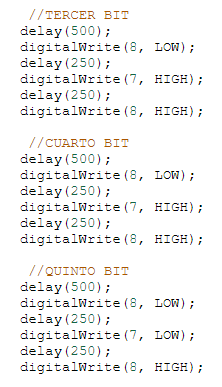
\includegraphics[width=5cm]{codigo_arduino1_2.PNG}
\centering
\caption{Segunda parte del código del Arduino transmisor.}
\label{fig:codigo_arduino1_2.PNG}
\end{figure}
\cite{punto2}\\

\newpage

\begin{figure}[h]
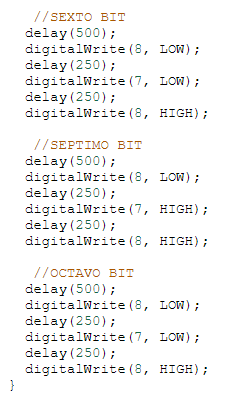
\includegraphics[width=5cm]{codigo_arduino1_3.PNG}
\centering
\caption{Tercera parte del código del Arduino transmisor.}
\label{fig:codigo_arduino1_3.PNG}
\end{figure}
\cite{punto2}\\


\newpage


\begin{figure}[h]
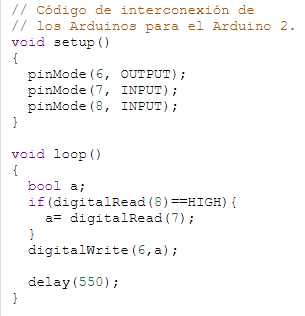
\includegraphics[width=6cm]{codigo_arduino2.PNG}
\centering
\caption{código del Arduino receptor.}
\label{fig:codigo_arduino2.PNG}
\end{figure}
\cite{punto2}\\


\subsection{Sistema de desencriptación.}

Para el sistema de desencriptación se utiliza un circuito integrado 74HC04 y dos 74HC08, los cuales corresponden a un circuito integrado de compuertas inversoras y de compuertas AND respectivamente.\\

Se usan 3 compuertas inversoras y 7 compuertas AND, siguiendo el esquema de la figura 8. Se utilizaron compuertas AND debido a que estas son compuertas que sólo obtienen un '1' para un caso, por lo que para otros casos en que no sean el solicitado arrojan '0'.


\begin{figure}[h]
\includegraphics[width=6cm]{compuertas_sistema_desencriptación.PNG}
\centering
\caption{Comopuertas del sistema de desencriptación.}
\label{fig:compuertas_sistema_desencriptación.PNG}
\end{figure}

El esquema de arduino para la implementación del esquema de la figura anterior junto con las compuertas lógicas es el de la figura 9, y el código que se implementó para observar el buen funcionamiento del circuito es el de la figura 10, en el cual se mandan los bits correspondientes a la clave individual del grupo, el número 171, el cual en bits corresponde al 10101011.


\begin{figure}[h]
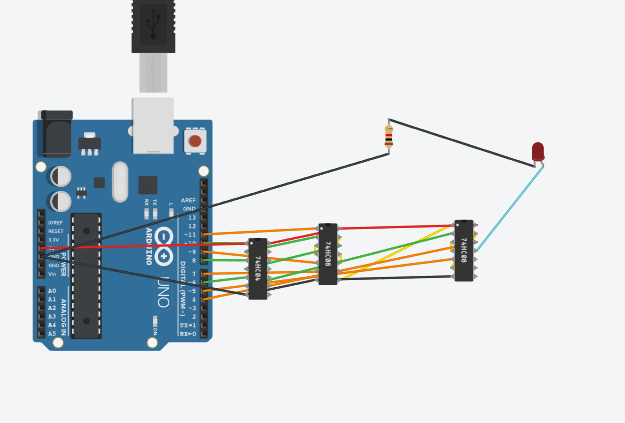
\includegraphics[width=6cm]{sistema_desencriptacion.PNG}
\centering
\caption{Sistema de desencriptación mediante compuertas lógicas.}
\label{fig:sistema_desencriptacion.PNG}
\end{figure}
\cite{punto3}\\

\begin{figure}[h]
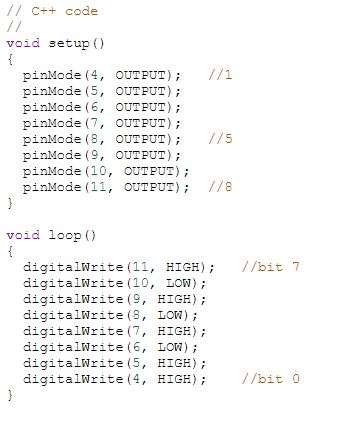
\includegraphics[width=7cm]{Desencrip1.JPG}
\centering
\caption{Código de prueba para la bandera del sistema de desencriptación.}
\label{fig:Desencrip1.PNG}
\end{figure}
\cite{punto3}\\

\newpage


\subsection{Sistema completo}

\subsubsection{Arduino transmisor}

Para el arduino transmisor, se utilizaron 3 salidas, correspondientes a la señal de datos (pin 8), señal de reloj (pin 7) y una señal que se activa antes del noveno flanco de subida de la señal de reloj y se desactiva 25 milisegundos después (pin 6).\\

\newpage

\begin{figure}[h]
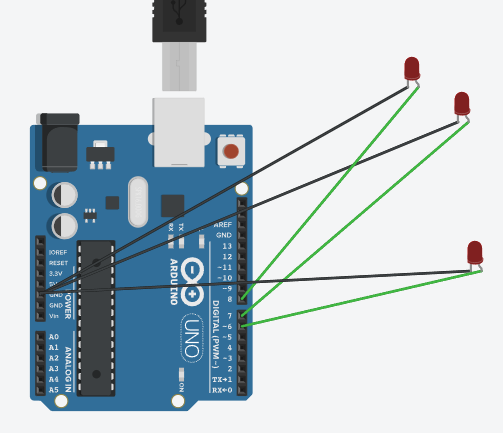
\includegraphics[width=6cm]{arduino_transmisor.PNG}
\centering
\caption{Circuito con Arduino configurado como transmisor.}
\label{fig:arduino_transmisor.PNG}
\end{figure}
\cite{punto41}\\

La señal del pin 8 es la señal que entrega los datos en bits de los valores del arreglo entregado. La señal del pin 7 (señal de reloj) controla el almacenamiento de cada bit de la señal de datos, y la señal del pin 6 controla la señal que se ingresa al circuito integrado 74HC595 que da cuenta de cuándo se deben enviar los bits almacenados a la salida del integrado en forma paralela. La realización de estas señales se observa en el código para el circuito de transmisión en las figuras 12 y 13. Se tiene en cuenta que la señal de datos debe tomar el valor deseado antes del flanco de subida del reloj, para esta se almacene adecuadamente, y que la señal del pin 6 debe generarse antes del noveno flanco de subida de la señal del reloj, para mostrar la cadena de 8 bits antes de recoger el noveno dato.\\

\newpage

\begin{figure}[h]
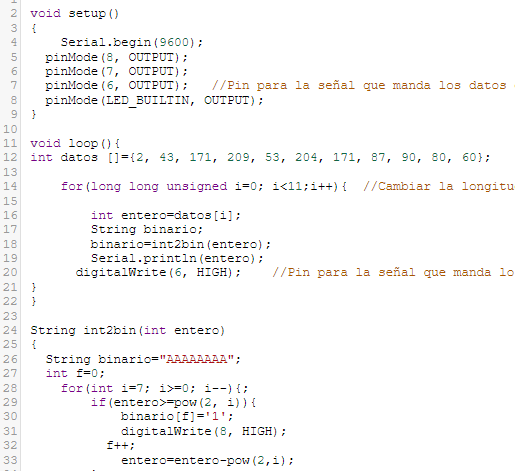
\includegraphics[width=9cm]{codigo_transmisor_1.PNG}
\centering
\caption{Primera parte del código del Arduino transmisor.}
\label{fig:codigo_transmisor_1.PNG}
\end{figure}
\cite{punto41}\\

\newpage

\begin{figure}[h]
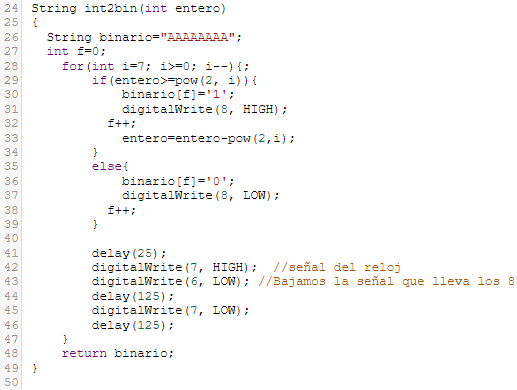
\includegraphics[width=9cm]{codigo_transmisor_2.PNG}
\centering
\caption{Segunda parte del código del Arduino transmisor.}
\label{fig:codigo_transmisor_2.PNG}
\end{figure}

Los datos importantes del código del arduito transmisor son la función int2bin (figura 13), la cual recoge el entero y lo transforma en string por medio de un for, el cual evalúa si su valor es mayor o igual a 2 a la séptima potencia, de ser así, se obtendrá un bit '1' en el bit más significativo. Así mismo se realizan con los demás bits. Además, en esta misma función se mandará por medio del puerto 8 el bit correspondiente a '1' o a '0' según es el caso. Al final de cada iteración del for, por tanto de cada envío de señal del dato en el puerto 8, se hace un delay de 25 milisegundos para generar la señal de subida del reloj. Además, al salir de la función (figura 12) se realiza el envío de la señal del puerto 6, para dar cuenta de que ya se cumplieron los envíos de los 8 bits.\\

Por medio de las 3 señales antes mensionadas y de la forma antes explicada se realiza una toma adecuada de los datos para el funcionamiento adecuado del circuito integrado 74HC595 y del arduino receptor.\\

\newpage

\subsubsection{Arduino transmisor y Circuito 74HC595}


\begin{figure}[h]
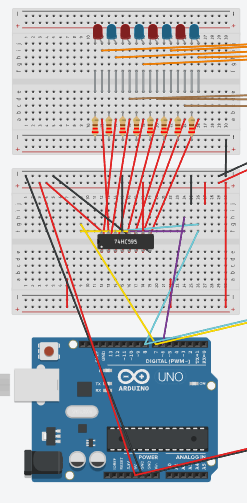
\includegraphics[width=4cm]{conexion_arduino_con_74HC595.PNG}
\centering
\caption{Conexión entre el Arduino transmisor y el circuito integrado 74HC595.}
\label{fig:conexion_arduino_con_74HC595.PNG}
\end{figure}
\cite{completo}\\

En la interconexión del arduino con el circuito integrado 74HC595, se interconectar el pin 8, 7 y 6 del arduino con los pines 14, 11 y 12 del 74HC595 respectivamente.\\

Se agregan LEDs para observar la serie de bits que arroja el integrado. Estos bits están ordenados por orden de peso de bit.

\subsubsection{Integrado 74HC595 y circuito de desencriptación}

Para realizar el circuito de desencriptación, se sigue el esquema de la figura 15. Se modifica este esquema respecto al numeral 1 en que se cambia un circuito de 4 AND de 2 entras (74HC08) por un circuito de 2 AND de 4 entradas (74HC21).

\newpage

\begin{figure}[h]
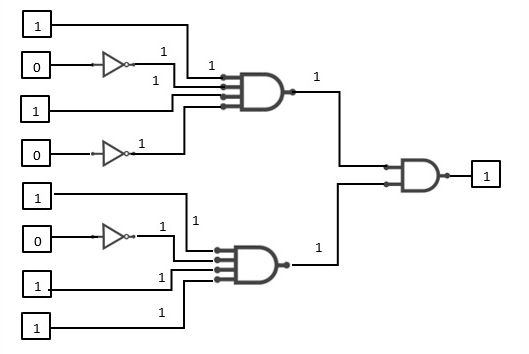
\includegraphics[width=6cm]{compuertas_sistema_completo.PNG}
\centering
\caption{Compuertas lógicas para el sistema completo.}
\label{fig:compuertas_sistema_completo.PNG}
\end{figure}
\cite{completo}\\

La conexión del circuito integrado 74HC595 y del sistema de desencriptación se observa en la figura 16, en donde se observa con cables cafés que los bits 1, 3 y 5 (derecha a izquierda) se dirigen al integrado correspondiente al de las compuertas lógicas inversoras. Esto es lo observado en el esquema de la figura anterior.


\begin{figure}[h]
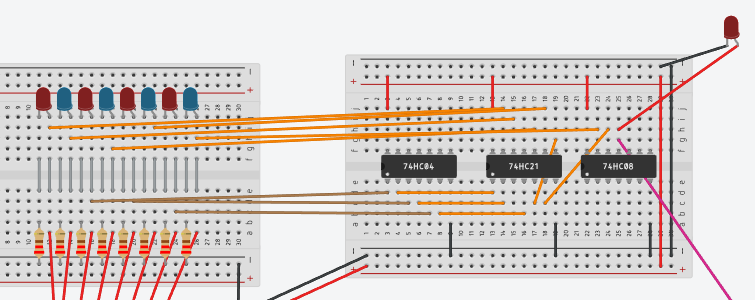
\includegraphics[width=9cm]{74HC595 y sistema desencriptacion.PNG}
\centering
\caption{Interconexión del sistema de paralelización y del sistema de desencriptación.}
\label{fig:74HC595 y sistema desencriptacion.PNG}
\end{figure}
\cite{completo}\\

Se agregó un LED a la señal de salida del esquema para comprobar el valor de la bandera. Esto se observa en la figura 16.

\newpage
\subsubsection{Arduino receptor}


\begin{figure}[h]
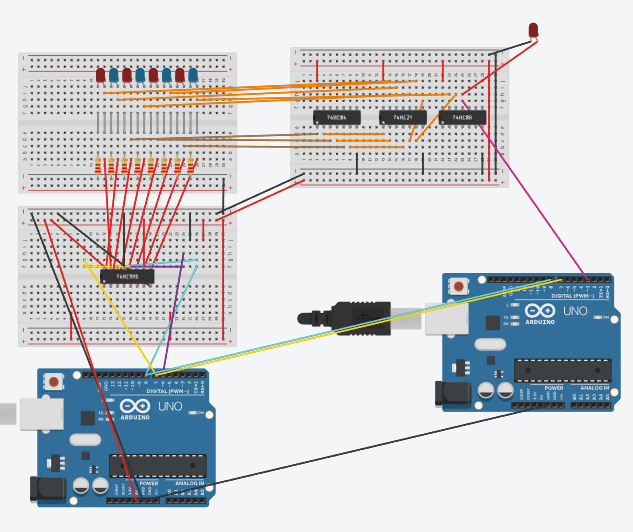
\includegraphics[width=7cm]{sistema_completo.PNG}
\centering
\caption{Sistema completo.}
\label{fig:sistema_completo.PNG}
\end{figure}
\cite{completo}\\


El Arduino receptor es el encargado de realizar el proceso en el que se identifica cual es el número mayor entre los últimos 5 números antes de que aparezca la bandera, es por ello por lo que el código del Arduino receptor es el observado en las figuras 18, 19 y 20:\\

\newpage

\begin{figure}[h]
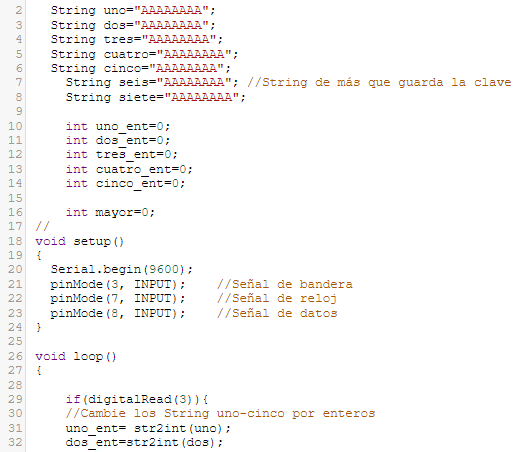
\includegraphics[width=9cm]{codigo_receptor_1.PNG}
\centering
\caption{Primera parte del código del Arduino receptor. }
\label{fig:codigo_receptor_1.PNG}
\end{figure}
\cite{completo}\\

\newpage
\begin{figure}[h]
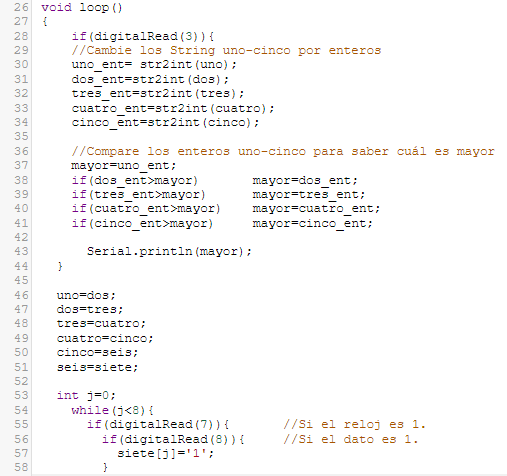
\includegraphics[width=9cm]{codigo_receptor_2.PNG}
\centering
\caption{Segunda parte del código del Arduino receptor. }
\label{fig:codigo_receptor_2.PNG}
\end{figure}
\cite{completo}\\

\newpage

\begin{figure}[h]
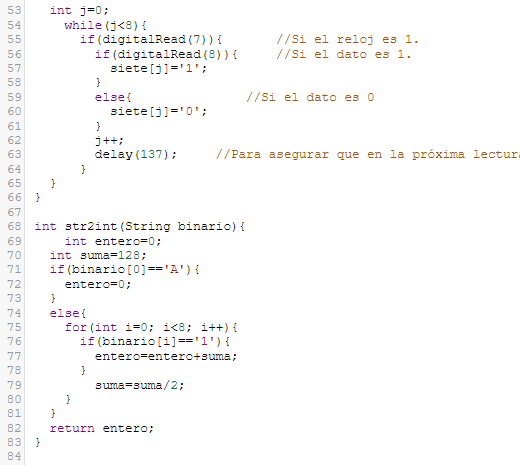
\includegraphics[width=9cm]{codigo_receptor_3.PNG}
\centering
\caption{Tercera parte del código del Arduino receptor. }
\label{fig:codigo_receptor_3.PNG}
\end{figure}
\cite{completo}\\


La estructura del circuito receptor es la siguiente:\\

Inicialmente hay siete variables tipo string almacenadas en cada una de ellas la letra \textit{‘A’}, 8 veces, con el fin de capturar los 8 bits de entrada de cada dato; es decir, las primeras variables se crean para almacenar 5 datos antes de que aparezca la bandera, el string seis se crea para almacenar la clave, y el string siete almacena el dato posterior a la clave. El dato, como se mencionó antes, es 171. \\

En la función \textit{setup} en el código de Arduino se inicializa la comunicación serial, se define los pines 3, 7, 8 como entrada que corresponde a la señal de bandera, de reloj y de datos respectivamente. En la función \textit{loop} se observa si el bit de la bandera está en '1'. De ser así, se cambia el tipo de dato de los datos de string a entero (de las variables de uno a siete a las de uno-ent a siete-ent) con la función str2int, y posteriormente se hacen una serie de if para tomar el valor de la variable mayor. En la función de str2int se toma en cuenta que los strings que no tengan bits sino un 'A' toma el valor de entero de 0, para que al comparar con el valor más grande este no se tome en cuenta.\\

Fuera de la condición de que la bandera sea '1', se realiza la toma de datos. Para esto, primero se trasladan las variables, para actualizar el dato más actual y desechar el dato más antiguo. Mediante un ciclo \textit{while} se establece la simulación del reloj y se toma los datos en cada flanco de subida, generando un delay de 550 milisegundos para dar el espacio de tiempo pertinente para que el reloj vuelva al valor de bajo y así almacenar en la variable siete el dato de entrada; esto se realiza comparando si lo que llega es un '1' o '0', y este valor se agrega en la posición pertinente del string siete.


\section{CONCLUSIONES} \label{conclulsion}
\begin{itemize}
\item La plataforma de Tinkercad, el microcontrolador Arduino, el lenguaje C++ y el circuito integrado 74HC575 son piezas claves tanto para la realización de este proyecto como para la realización de otros proyectos prácticos.

\item El microcontrolador Arduino es útil para el envío y recepción de información a diferentes sistemas y también a otros arduinos.

\item En un sistema de transmisión y recepción de datos, es importante tener una señal de reloj que de cuenta del dato presente.

\item En el sistema de comunicación, los datos generados deben producirse antes del flanco de referencia del reloj, para asegurar que estos datos sean los correctos, ya que si se genera al mismo tiempo del flanco del reloj, puede tomar el dato anterio y no el actual.

\item La señal del pin 6 se debe generar antes del noveno flanco de subida de la señal del reloj, para mostrar la cadena de 8 bits antes de que el reloj recoga el dato del noveno bit.

\item El uso del circuito integrado 74HC595 es útil para el envío paralelo de los datos en sus 8 puertos de salida.

\item El arduino se programa en lenguaje de C++, siempre y cuando se respeten funciones principales setup y loop del arduino.

\item Con las compuertas lógicas se pueden crear sistemas para el reconocimiento de bits especificados.



\end{itemize}

\section{REFERENCIAS}    

\bibliographystyle{IEEEtran}

\bibliography{references}

\end{document}
